%for compilation: xelatex psi_2015.tex 
\documentclass{llncs}

\usepackage{makeidx}  % allows for indexgeneration
\usepackage{listings}
\usepackage{algpseudocode}
\usepackage{algorithm}
\usepackage{caption}
\usepackage{algorithmicx}
\usepackage{mathspec}
\usepackage{textcomp}
%\usepackage{subcaption}
\usepackage{subfig} 

\begin{document}

\algtext*{EndWhile}% Remove "end while" text
\algtext*{EndIf}% Remove "end if" text
\algtext*{EndFor}% Remove "end for" text
\algtext*{EndFunction}% Remove "end function" text

\frontmatter          % for the preliminaries

\pagestyle{headings}  % switches on printing of running heads
\addtocmark{Hamiltonian Mechanics} % additional mark in the TOC

\title{Relaxed Parsing for Regular Approximations of String-Embedded Languages}
\titlerunning{Relaxed Parsing for Regular Approximations of String-Embedded Languages}  % abbreviated title (for running head)


\author{Ekaterina Verbitskaia\inst{1} \and Semyon Grigorev\inst{2}
\and Dmitry Avdyukhin\inst{3}}
%
%\authorrunning{Ivar Ekeland et al.} % abbreviated author list (for running head)
%

\institute{Saint Petersburg State University\\
\email{kajigor@gmail.com},
\and
\email{rsdpisuy@gmail.com}
\and
\email{dimonbv@gmail.com}}

\maketitle              % typeset the title of the contribution

%%
%% The abstract is a short summary of the work to be presented in the
%% article.
\begin{abstract}
В последнее время наблюдается рост интереса к решению задач, связанных с контекстно-свободными запросами на графах.
Критически важной становится потребность в измерении производительности алгоритмов решающих подобные задачи.
Тем не менее разработка наборов контрольных данных и стандартизированные процедуры оценки отстают, что препятствует продвижению вперед в этой области.
Чтобы решить эти проблемы мы представляем коллекцию CFPQ\_Data, в которой собраны наиболее популярные графы для проведения экспериментального анализа алгоритмов решающих задачи контекстно-свободных запросов на графах.
Коллекция состоит из более чем 40 графов разного размера.
Также мы предоставляем загрузчики данных и реализации наиболее популярных алгоритмов на основе Python, а также стандарт проведения экспериментов и базовых показателей работы алгоритма.
Здесь мы даем обзор собранной коллекции, стандартизированных процедур исследования и проводим базовые эксперименты.
Все наборы данных доступны на сайте \href{https://github.com/JetBrains-Research/CFPQ_Data}{https://github.com/JetBrains-Research/CFPQ\_Data}.
Проведенные эксперименты полностью воспроизводимы из кода, доступного на сайте \href{https://github.com/JetBrains-Research/CFPQ_PyAlgo}{https://github.com/JetBrains-Research/CFPQ\_PyAlgo}.
\end{abstract}

\section{Introduction}

Scalable high-performance graph analysis is an actual challenge.
There is a big number of ways to attack this challenge~\cite{Coimbra2021} and the first promising idea is to utilize general-purpose graphic processing units (GPGPU).
Such existing solutions, as CuSha~\cite{10.1145/2600212.2600227} and Gunrock~\cite{7967137} show that utilization of GPUs can improve the performance of graph analysis, moreover it is shown that solutions may be scaled to multi-GPU systems.
But low flexibility and high complexity of API are problems of these solutions.

The second promising thing which provides a user-friendly API for high-performance graph analysis algorithms creation is a GraphBLAS API~\cite{7761646} which provides linear algebra based building blocks to create graph analysis algorithms.
The idea of GraphBLAS is based on a well-known fact that linear algebra operations can be efficiently implemented on parallel hardware.
Along with that, a graph can be natively represented using matrices: adjacency matrix, incidence matrix, etc.
While reference CPU-based implementation of GraphBLAS, SuiteSparse:GraphBLAS~\cite{10.1145/3322125}, demonstrates good performance in real-world tasks, GPU-based implementation is challenging.

One of the challenges in this way is that real data are often sparse, thus underlying matrices and vectors are also sparse, and, as a result, classical dense data structures and respective algorithms are inefficient. 
So, it is necessary to use advanced data structures and procedures to implement sparse linear algebra, but the efficient implementation of them on GPU is hard due to the irregularity of workload and data access patterns.
Though such well-known libraries as cuSPARSE show that sparse linear algebra operations can be efficiently implemented for GPGPU, it is not so trivial to implement GraphBLAS on GPGPU. 
First of all, it requires \textit{generic} sparse linear algebra, thus it is impossible just to reuse existing libraries which are almost all specified for operations over floats.
The second problem is specific optimizations, such as masking fusion, which can not be natively implemented on top of existing kernels.
Nevertheless, there is a number of implementations of GraphBLAS on GPGPU, such as GraphBLAST~\cite{yang2019graphblast}, GBTL~\cite{7529957}, which show that GPGPUs utilization can improve the performance of GraphBLAS-based graph analysis solutions.
But these solutions are not portable because they are based on Nvidia Cuda stack.
Moreover, the scalability problem is not solved: all these solutions support only single-GPU, not multi-GPU computations.

To provide portable GPU implementation of GraphBLAS API we developed a \textit{SPLA} library\footnote{Source code available at: \url{https://github.com/JetBrains-Research/spla}}.
This library utilizes OpenCL for GPGPU computing to be portable across devices of different vendors.
Moreover, it is initially designed to utilize multiple GPGPUs to be scalable.
To sum up, the contribution of this work is the following.
\begin{itemize}
    \item Design of portable GPU GraphBLAS implementation proposed. The design involves the utilization of multiple GPUS. Additionally, the proposed design is aimed to simplify library tuning and wrappers for different high-level platforms and languages creation. 
    \item Subset of GraphBLAS API, including such operations as masking, matrix-matrix multiplication, matrix-matrix e-wise addition, is implemented. The current implementation is limited by COO and CSR matrix representation format and uses basic algorithms for some operations, but work in progress and more data formats will be supported and advanced algorithms will be implemented in the future.
    \item Preliminary evaluation on such algorithms as breadth-first search (BFS) and triangles counting (TC), and real-world graphs shows portability across different vendors and promising performance: for some problems Spla is comparable with GraphBLAST. Surprisingly, for some problems, the proposed solution on embedded Intel graphic card shows better performance than SuiteSparse:GraphBLAS on the respective CPU. At the same time, the evaluation shows that further optimization is required.
\end{itemize} 
\section{Related Works}

Our parsing algorithm is based on a RNGLR-algorithm presented by Elizabeth Scott 
and Adrian Johnstone in~\cite{RNGLR}. In order to better understand the paper, a reader 
should be familiar to its principles of work, so we briefly describe RNGLR-algorithm 
in this section.  Also we point out differences between our approach and existing
tools which operate with regular approximation of string-embedded language since
we use such type of approximation as input for our algorithm.

% Abstract parsing -- Doh

\subsection{Regular Approximation of Sting-Embedded Language}
Some tools are aimed to build high quality regular approximation. For example, 
Stranger~\cite{Stranger} which use forward reachability analysis to compute 
over-approximation of all string values for program. Further analysis in Stranger 
is based on patterns detection in approximation or generation finite subset of 
strings for analyzing with standalone tools. Implementation of our algorithm may 
use such tools as input generator.

Paper~\cite{JSA} presents Java String Analyzer (JSA) � tool for static syntax 
correctness checking of embedded SQL statements.  This tool build regular approximation 
with Mohri-Nederhof~\cite{MohriNederhof} algorithm and then check its inclusion into reference grammar 
without parsing and forest construction.
 
Our algorithm is inspired by Alvor~\cite{Alvor} which apply GLR-based technique 
for syntax correctness checking of regular approximation. Key difference of our 
algorithm is building of parse forest finite representation. 

\subsection{RNGLR}
Generalized LR parsing algorithm was presented by Masaru Tomita~\cite{Tomita}
as a solution for natural language processing and was intended to handle ambiguous
context-free grammars. Ambiguities of grammar produce Shift/Reduce and 
Reduce/Reduce conflicts. The algorithm uses parser tables similar to classical LR-tables,
each cell of which can contain multiple actions in case of conflicts. The general approach of 
the algorithm is to carry out all possible actions in these situations. 

However, Tomita's algorithm failed to process general context-free grammars.  
Elizabeth Scott and Adrian Johnstone presented Right-Nulled Generalized LR algorithm~\cite{RNGLR}
which extends and corrects Tomita's GLR parsing methods by
specific way of handling \emph{right nullable} rules (i.e. rules of the form 
$\mathrm{A} \rightarrow \alpha \beta$, where $\beta$ reduces to the empty string). 
That is, not only reductions for items $\mathrm{A} \rightarrow \alpha \cdot$ are 
applied, but also for the items of the form  $\mathrm{A} \rightarrow \alpha \cdot 
\beta$, where $\beta \Rightarrow \epsilon$. Thus, reduction length -- the number of 
symbols to be reduced to a nonterminal -- may be less than or equal to the length 
of righthand side of the rule. There are also possible reductions of 0-length, 
also called as $\epsilon$-reductions, corresponding to items of the form $\mathrm{A} 
\rightarrow \cdot$. 

To represent the set of stacks produced during conflict processing efficiently,
RNGLR algorithm uses Graph Structured Stack. GSS is an ordered graph, 
vertices of which corresponds to elements of classical stack and edges link sequential 
elements together. Each vertex can have multiple incoming edges and by means of 
it be shared between several stacks. Vertex is a pair $(s, l)$, where $s$ is a 
parser state and $l$ is a level -- position in an input string. Vertices in GSS 
are unique and there is no multiple edges. GSS construction routine is illustrated with 
\emph{addVertex} and \emph{addEdge} functions in Algorithm~\ref{rnglr}.

RNGLR-algorithm reads an input from left to right, one token at a time, and 
constructs levels of GSS sequentially for each position in the input. In the 
main loop of the algorithm for each token from the input, firstly, all possible 
reductions are applied (see \emph{reduce} function in Algorithm~\ref{rnglr}), and then the next token 
is shifted (see \emph{push} function in Algorithm~\ref{rnglr}).
\begin{algorithm}[!ht]
\begin{algorithmic}[1]
\caption{RNGLR algorithm}
\label{rnglr}
  
\Function{addVertex}{$level, state$}
  \If{GSS does not contain vertex $v = (level, state)$}
    \State{add new vertex $v = (level, state)$ to GSS}
    \State{calculate the set of shifts by $v$ and the next token and add them to $\mathcal{Q}$}
    \State{calculate the set of zero-reductions by $v$ and the next token and add them to $\mathcal{R}$}
  \EndIf
  \State{\Return{$v$}}
\EndFunction

\Function{addEdge}{$v_{h}, level_{t}, state_{t}, isZeroReduction$}
  \State{$v_{t} \gets$ \Call{addVertex}{$level_{t}, state_{t}$}}
  \If{GSS does not contain edge from $v_{t}$ to $v_{h}$}
    \State{add new edge from $v_{t}$ to $v_{h}$ to GSS}
    \If{not $isZeroReduction$}
      \State{calculate the set of reductions by $v$ and the next token and add them to $\mathcal{R}$}
    \EndIf
  \EndIf
\EndFunction

\Function{reduce}{}
  \While{$\mathcal{R}$ is not empty}
    \State{$(v, N, l) \gets \mathcal{R}.Dequeue()$}
    \State{find the set $\mathcal{X}$ of vertices reachable from $v$ along the path of length $(l-1)$, or length $0$ if $l=0$}
    \ForAll{$v_{h} = (level_{h}, state_{h})$ in $\mathcal{X}$}
      \State{$state_{t} \gets$ calculate new state by $state_{h}$ and nonterminal $N$}
      \State{\Call{addEdge}{$v_{h}, v.level, state_{tail}, (l=0)$}}
    \EndFor
  \EndWhile
\EndFunction

\Function{push}{}
  \State{$\mathcal{Q^{'}} \gets$ copy $\mathcal{Q}$}
  \While{$\mathcal{Q^{'}}$ is not empty}
    \State{$(v, state) \gets \mathcal{Q}.Dequeue()$}
    \State{\Call{addEdge}{$v, v.level + 1, state, false$}}
  \EndWhile
\EndFunction

\end{algorithmic}
\end{algorithm}

\section{Механизм диагностики ошибок}
Предлагаемый механизм диагностики ошибок состоит из двух частей:
\begin{itemize}
    \item алгоритм синтаксического анализа регулярной аппроксимации динамически формируемых выражений (далее основной анализ) модифицируется, позволяя для каждой GSS вершины строить все корректные для нее префиксы внутреннего графа;
    \item после основного анализа с помощью построенных префиксов обнаруживаются ошибочные ребра внутреннего графа.
\end{itemize}
Далее в этой главе будут рассмотрены: компактное представление префиксов внутреннего графа, алгоритм построения корректных префиксов внутреннего графа для GSS-вершин и алгоритм диагностики ошибок, проводящий анализ построенных префиксов.

\subsection{Компактное представление префиксов внутреннего графа}
Так как внутренний граф может иметь циклы, то множество различных префиксов внутреннего графа может быть бесконечным. В качестве компактного представления всех корректных префиксов внутреннего графа для вершины GSS используется ориентированный граф с выделенным множеством начальных вершин (далее \emph{граф префиксов}). Из-за особенностей операций, используемых при построении графов префиксов, начальные вершины представляют не начало, а конец хранимых префиксов внутреннего графа в рассматриваемом графе префиксов. Каждая вершина в графе префиксов ассоциируется с ребром GSS или является специальной вершиной $EOP$ (End Of Prefix). Ребра GSS, в свою очередь, будем делить на три вида:
\begin{itemize}
    \item  \emph{терминальное} ребро --- ребро, порожденное операцией сдвига по какому-то терминалу $t$;
    \item \emph{нетерминальное} --- ребро, порожденное операцией свертки длины $l$, где $l > 0$;
    \item \emph{обнуляемое} --- ребро, порожденное операцией свертки длины $l$, где $l = 0$.
\end{itemize}
Будем говорить, что начальная вершина $V$ графа префиксов $GP_{1}$ \emph{соединена} с графом префиксов $GP_{2}$, если для любой начальной вершины $U$ графа префиксов $GP_{2}$, существует ребро из вершины $V$ в вершину $U$. Каждая, кроме $EOP$, начальная вершина графа префиксов соединена с одним графом префиксов. Вершина $EOP$ не имеет исходящих дуг.

С каждым нетерминальным ребром ассоциируется множество путей в GSS, по которым произведена операция свертки для данного нетерминального ребра. Будем говорить что данное нетерминальное ребро \emph{порождает} каждый путь из рассмотренного множества путей GSS.
% * <Екатерина Вербицкая> 14:16:56 13 May 2016 UTC+0300:
% > множество путей в GSS, по которым произведена операция свертки
% 
% Я не уверена, что так говорить корректно.

Рассмотрим путь $(V_{1},..,V_{n})$ в графе префиксов $GP$ как последовательность вершин графов префиксов. Удалим вершину $EOP$, если она присутствует, а также заменим все вершины в данном пути на ребра GSS, с которыми они ассоциируются. Получим последовательность $(e_{1},..,e_{n})$ ребер GSS. \emph{Раскрытием} данной последовательности будем называть последовательность, получающуюся в результате применения следующих действий:
\begin{itemize}
    \item все нетерминальные ребра GSS $e$, заменяются на последовательность ребер, соответствующую одному из порожденных ребром $e$ пути;
    \item все обнуляемые ребра GSS удаляются из последовательности.
\end{itemize}
Если после конечного числа раскрытий в последовательности останутся только терминальные ребра GSS, то будем говорить, что изначальный путь в графе префиксов \emph{сводится} к строке, получающейся инвертированием этой последовательности терминальных ребер и их замены на терминалы, с которыми они ассоциированы. Если полученная строка получается заменой ребер в пути префикса внутреннего графа $P$, на терминалы, которыми нагружены эти ребра, то путь в графе префиксов \emph{сводится} к префиксу внутреннего графа $P$. Будем говорить, что граф префиксов $GP$ \emph{порождает} префикс внутреннего графа $P$, если $\exists (V_{1},..,V_{n},EOP)$ --- путь в графе префиксов $GP$, где $V_{1}$ --- одна из начальных вершин графа префиксов $GP$, который сводится к префиксу внутреннего графа $P$. В графе префиксов также могут быть циклы, что позволяет сводиться к бесконечному множеству префиксов внутреннего графа.
% * <Екатерина Вербицкая> 14:24:18 13 May 2016 UTC+0300:
% Сюда бы тоже картинку.

\subsection{Алгоритм построения префиксов}
Данный алгоритм является модификацией алгоритма ослабленного синтаксического анализа регулярной аппроксимации динамически формируемого выражения. Добавляется ассоциация вершин GSS с коллекцией $prefixes$ --- граф префиксов, порождающий все корректные префиксы внутреннего графа для данной GSS вершины. После создания начальной GSS-вершины в ее графе префиксов создается начальная вершина $EOP$. Добавляется ассоциация нетерминальных ребер GSS с коллекцией $paths$ --- множество путей в GSS, порождаемых рассматриваемым нетерминальным ребром. Функция $addEdge$ модифицируется, добавляется дополнительный параметр $pathsToAdd$ --- множество путей в GSS, которое необходимо добавить к множеству путей в GSS, порождаемых ребром $edge$ из вершины $v_{t}$ в вершину $v_{h}$. Также создается начальная вершина графа префиксов $v_{t}.prefixes$, ассоциированная с ребром $edge$ и соединенная с графом префиксов $v_{h}.prefixes$. Функция $addVertex$ не изменилась.

\begin{algorithm}[H]
\begin{algorithmic}[1]
\caption{Модификация построения GSS}
\label{addEdge_mod}
\Function{addEdge}{$v_{h}, innerGraphV, state_{t}, isZeroReduction, pathsToAdd$}

  \State{$(v_{t}, isNew) \gets$ \Call{addVertex}{$innerGraphV, state_{t}$}}
  \If{GSS does not contain edge from $v_{t}$ to $v_{h}$}
% * <Екатерина Вербицкая> 14:26:52 13 May 2016 UTC+0300:
% Может тут тоже можно половину кода выкинуть, оставив только важное.
% ^ <Рустам Азимов> 14:27:51 13 May 2016 UTC+0300:
% Не представляю пока. Как это?
    \State{$edge \gets$ create new edge from $v_{t}$ to $v_{h}$}
    \State{$\mathcal{Q}.Enqueue(innerGraphV)$}
    \If{not $isNew$ and $v_{t}.passingReductions.Count>0$}
      \State{add $(v_{t}, edge)$ in $innerGraphV.passingReductionsToHandle$}
    \EndIf
    \If{not $isZeroReduction$}
      \ForAll{$e$ in outgoing edges of $innerGraphV$}
        \State{calculate the set of reductions by $v$ and the token on $e$}
        \State{     and add them in $innerGraphV.reductions$}
      \EndFor
    \EndIf
    \State{$V \gets$ vertex of the prefix graph,}
    \State{     associated with $edge$ and connected to $v_{h}.prefixes$}
    \State{add $V$ to initial vertexes of $v_{t}.prefixes$}
  \EndIf
  \If{pathsToAdd is not empty}
    \State{$edge \gets$ edge from $v_{t}$ to $v_{h}$}
    \State{add all paths in $pathsToAdd$ to $edge.paths$}
  \EndIf
\EndFunction
\end{algorithmic}
\end{algorithm}

Параметр $pathsToAdd$ при вызове функции $addEdge$ для терминальных или обнуляемых ребер GSS является пустым множеством.

\begin{algorithm}[H]
\begin{algorithmic}[1]
\caption{Модификация операции сдвига}
\label{push_mod}
\Function{push}{$innerGraphV$}
  \State{$\mathcal{U} \gets$ copy $innerGraphV.unprocessed$}
  \State{clear $innerGraphV.unprocessed$}
  \ForAll{$v_{h}$ in $\mathcal{U}$}  
    \ForAll{$e$ in outgoing edges of $innerGraphV$}
      \State{$push \gets$ calculate next state by $v_{h}.state$ and the token on $e$}
      \State{$pathsToAdd \gets$ empty set}
% * <Екатерина Вербицкая> 14:32:07 13 May 2016 UTC+0300:
% Обычно в таких листингах новый код выделяется болдом или еще как-то в том же духе. Чтобы повысить читабельность и чтобы сразу было понятно, что конкретно изменилось.
      \State{\Call{addEdge}{$v_{h}, e.Head, push, false, pathsToAdd$}}
      \State{add $v_{h}$ in $innerGraphV.processed$}
    \EndFor
  \EndFor
\EndFunction
\end{algorithmic}
\end{algorithm}

\begin{algorithm}[H]
\begin{algorithmic}[1]
\caption{Модификация операции свертки}
\label{reduce_mod}
\Function{makeReductions}{$innerGraphV$}
  \While{$innerGraphV.reductions$ is not empty}
    \State{$(startV, N, l) \gets innerGraphV.reductions.Dequeue()$}
    \State{find the set of vertices $\mathcal{X}$ reachable from $startV$}
    \State{    along the path of length ($l-1$), or $0$ if $l=0$;}
    \State{add $(startV, N, l-i)$ in $v.passingReductions$,}
    \State{    where $v$ is an $i$-th vertex of the path}
    \ForAll{$v_{h}$ in $\mathcal{X}$}
      \State{$state_{t} \gets$ calculate new state by $v_{h}.state$ and nonterminal $N$}
      \If{$l > 0$}
        \State{$pathsToAdd \gets$ all paths, by which $v_{h}$ is reachable}
        \State{     from $startV$}
      \Else
        \State{$pathsToAdd \gets$ empty set}
      \EndIf
      \State{\Call{addEdge}{$v_{h}, startV, state_{t}, (l=0), pathsToAdd$}}
    \EndFor
  \EndWhile
\EndFunction

\Function{applyPassingReductions}{$innerGraphV$}
  \ForAll{$(v, edge)$ in $innerGraphV.passingReductionsToHandle$}
    \ForAll{$(startV, N, l) \gets v.passingReductions.Dequeue()$}
      \State{find the set of vertices $\mathcal{X}$,}
      \State{    reachable from $edge$ along the path of length ($l-1$)}
      \ForAll{$v_{h}$ in $\mathcal{X}$}
        \State{$state_{t} \gets$ calculate new state by $v_{h}.state$ and nonterminal $N$}
        \State{$pathsToAdd \gets$ all paths, by which $v_{h}$ is reachable}
        \State{     from $startV$}
        \State{\Call{addEdge}{$v_{h}, startV, state_{t}, false, pathsToAdd$}}
      \EndFor
    \EndFor
  \EndFor
\EndFunction
\end{algorithmic}
\end{algorithm}

После описанных модификаций алгоритм синтаксического анализа регулярной аппроксимации динамически формируемого выражения для каждой вершины GSS дополнительно конструирует все корректные для нее префиксы внутреннего графа.

\subsection{Алгоритм диагностики ошибок}
Данный алгоритм получает на вход внутренний граф с построенными в ходе основного синтаксического анализа структурами (в том числе и префиксами внутреннего графа GSS вершин), а также сгенерированные RNGLR-таблицы. Алгоритм делает обход внутреннего графа и для каждого исходящего из вершины внутреннего графа ребра анализирует множества графов префиксов соседних вершин. 

Для обхода внутреннего графа используется глобальная очередь $Q$. Все ребра внутреннего графа, ведущие не в конечную вершину, обрабатываются в функции $processVertex$. Для ребер, ведущих в конечную вершину внутреннего графа, используется глобальная очередь $F$, с последующей обработкой в функции $processEOF$.

В результате работы алгоритма все ребра из множества $errors$ являются ошибочными, а ребра из множества $probErrors$ --- возможно ошибочными. То есть множество всех ошибочных ребер принадлежит объединению двух данных множеств. Кроме того, с элементами этих множеств ассоциируются множества графов префиксов (элемент $e$ множества $errors$ или множества $probErrors$ ассоциируется со множеством $errors[e]$ или $probErrors[e]$ соответственно), которые порождают корректные префиксы, заканчивающиеся в вершине, из которой исходит рассматриваемое ребро. Данные множества могут быть использованы при создании сообщения пользователю о возможных ошибках динамически формируемого выражения. Все префиксы, порождаемые графами префиксов из множества $errors[e]$, становятся некорректными при добавлении в конец ребра $e$. Все префиксы, порождаемые графами префиксов из множества $probErrors[e]$, возможно становятся некорректными при добавлении в конец ребра $e$. Но множество всех корректных префиксов внутреннего графа, заканчивающихся в вершине, из которой исходит ребро $e$, и становящихся некорректными при добавлении ребра $e$ в конец, порождается хотя бы одним графом префиксов из объединения множеств $errors[e]$ и $probErrors[e]$, где множество $errors[e]$ пусто, если $e \notin errors$, и множество $probErrors[e]$ пусто, если $e \notin probErrors$.
% * <Екатерина Вербицкая> 14:37:32 13 May 2016 UTC+0300:
% Что такое возможно ошибочные ребра? Почему множество всех ошибок -- это множество ошибок плюс возможно ошибочные?

\begin{algorithm}[H]
\begin{algorithmic}[1]
\caption{Алгоритм диагностики ошибок}
\label{error_handling}
\Function{findErrors}{$inputGraph, parserSource$}
    \State{$\mathcal{Q}.Enqueue(inputGraph.startVertex)$}
    \While{$Q$ is not empty}
        \State{$v \gets \mathcal{Q}.Dequeue()$}
        \State{\Call{processVertex}{$v$}}
    \EndWhile
    \While{$F$ is not empty}
        \State{$e \gets \mathcal{F}.Dequeue()$}
        \State{\Call{processEOF}{$e$}}
    \EndWhile
\EndFunction
\end{algorithmic}
\end{algorithm}

\begin{algorithm}[H]
\begin{algorithmic}[1]
\caption{Анализ неконечных ребер внутреннего графа}
\label{error_edges}
\Function{processVertex}{$innerGraphV$}
    \ForAll{$e$ in outgoing edges of $innerGraphV$}
        \If{token on $e$ is EOF}
            \State{$\mathcal{F}.Enqueue(e)$}
        \Else
            \If{$e.Head$ was not processed}
                \State{$\mathcal{Q}.Enqueue(e.Head)$}
            \EndIf
            \State{$headPrefixes \gets$ all prefixes graphs}
            \State{    from all GSS vertexes of $e.Head$;}
            \State{$pushedPrefixes \gets$ all prefixes graphs, to which connected}
            \State{    some initial vertex of prefixes graph in $headPrefixes$,}
            \State{     associated with terminal edge;}
            \State{$withCycle \gets$ all cyclical prefixes graphs in $pushedPrefixes$}
            \State{$withoutCycle \gets$ all non-cyclical graphs in $pushedPrefixes$}
            \State{$notPushedPrefixes \gets$ all prefixes graphs}
            \State{     from all GSS vertexes of $innerGraphV$,}
            \State{     without prefixes graphs from $pushedPrefixes$;}
            \ForAll{$p$ in $notPushedPrefixes$}
                \If{prefixes graph $p$ has a cycle}
                    \State{add $e$ to $probErrors$}
                    \State{add $p$ to $probErrors[e]$}
                \Else
                    \ForAll{$prefixPath$ in paths of prefixes graph $p$}
                        \State{$pathG \gets$ prefixes graph generated by $prefixPath$}
                        \If{$withoutCycle$ does not have any prefixes graph with
                            \State{    equivalent to $prefixPath$ path} }
                            \If{$withCycle$ is not empty}
                                \State{add $e$ to $probErrors$}
                                \State{add $pathG$ to $probErrors[e]$}
                            \Else
                                \State{add $e$ to $errors$}
                                \State{add $pathG$ to $errors[e]$}
                            \EndIf
                        \EndIf
                    \EndFor
                \EndIf
            \EndFor
        \EndIf
    \EndFor
\EndFunction
\end{algorithmic}
\end{algorithm}

\begin{algorithm}[H]
\begin{algorithmic}[1]
\caption{Анализ конечных ребер внутреннего графа}
\label{error_EOFedges}
\Function{processEOF}{$edge$}
    \State{$acceptedPrefixes \gets$ all prefixes graphs}
    \State{    from all GSS vertexes of $edge.Tail$ with accepted state;}
    \State{$withCycle \gets$ all cyclical prefixes graphs in $acceptedPrefixes$}
    \State{$withoutCycle \gets$ all non-cyclical graphs in $acceptedPrefixes$}
    \State{$notAcceptedPrefixes \gets$ all prefixes graphs}
    \State{    from all GSS vertexes of $edge.Tail$ with not accepted state;}
    \ForAll{$p$ in $notAcceptedPrefixes$}
        \If{prefixes graph $p$ has a cycle}
            \State{add $edge$ to $probErrors$} 
% * <Екатерина Вербицкая> 14:42:34 13 May 2016 UTC+0300:
% Вообще наличие цикла не говорит о том, что у нас обязательно в нем ошибка, поэтому нужна хоть какая-то мотивация в пользу такого подхода.
            \State{add $p$ to $probErrors[edge]$}
        \Else
            \ForAll{$prefixPath$ in paths of prefixes graph $p$}
                \State{$pathG \gets$ prefixes graph generated by $prefixPath$}
                \If{$withoutCycle$ does not have any prefixes graph 
                    \State{     with equivalent to $prefixPath$ path} }
                    \If{$withCycle$ is not empty}
                        \State{add $edge$ to $probErrors$}
                        \State{add $pathG$ to $probErrors[edge]$}
                    \Else
                        \State{add $edge$ to $errors$}
                        \State{add $pathG$ to $errors[edge]$}
                    \EndIf
                \EndIf
            \EndFor
        \EndIf
    \EndFor
\EndFunction
\end{algorithmic}
\end{algorithm}


\section{Correctness of the Algorithm}
\textsc{Theorem 1.}
\textit{For any given deterministic context-free grammar and any given nondeterministic
finite automaton with single start and single final state and with no $\epsilon$-transitions,
the algorithm terminates.}

\textsc{Proof.}
Each vertex of inner representation of the input finite automaton contains, at most, 
$N$ GSS vertices, where $N$ is a number of parser states, so for the inner graph which contains $n$
vertices, the number of GSS vertices is, at most, $Nn$. GSS has no multiple edges:
an edge $(v_{1}, v_{2})$ is only created if no edge exists between $v_{1}$ and $v_{2}$,  
meaning, the number of edges is limited with $(Nn) \cdot (Nn - 1) / 2 $. 

The algorithm dequeues vertex to be processed from the queue $Q$ at each iteration of the 
main loop. Vertices are enqueued to $Q$ only if new edge is added to GSS. As a number of 
GSS edges is finite, the algorithm always terminates. 

~\\
\textsc{Definition.} 
\emph{Correct tree} is an ordered, rooted tree with the following properties:
\begin{enumerate}
  \item The root is the start nonterminal of the grammar $G$
  \item The leaf nodes are the terminals of $G$. The sequence of the leaf nodes 
        corresponds to a path in the inner graph. 
  \item The interior nodes are the nonterminals of $G$. The children of nonterminal 
        $N$ correspond to the symbols on the righthand side of some production for $N$ in $G$.
\end{enumerate}

~\\
\textsc{Lemma 1.}
For every GSS edge $(v_{t}, v_{h})$, $v_{t} \in V_{t}.processed$, $v_{h} \in V_{h}.processed$, 
the terminals of the associated subtree corresponds to some path in the inner graph $p$ from $V_{h}$ to $V_{t}$

\textsc{Proof.}
The proof is by induction on the height of derivation tree. 
A tree of 0-height may be either an $\epsilon$-tree or a tree of a single leaf.
An $\epsilon$-tree corresponds to a path of 0-lenght, the tail and the head of the edge associated with 
$\epsilon$-tree are identical, thus the statement is true. A tree of a single leaf corresponds to a single 
terminal read from an edge ($V_{h}$, $V_{t}$) of the inner graph, thus the statement is true.

A tree which has height $k$ has a nonterminal $N$ as a root. By third item in the definition of correct tree, 
there is a production $N \rightarrow A_{0}, A_{1} \dots A_{n}$ for children of the root $A_{0}, A_{1} \dots A_{n}$. 
Subtree $A_{i}$ is associated with the GSS edge $(v_{t}^{i}, v_{h}^{i})$ and as its height is $k-1$, by induction,
there is a path in the inner graph from $V_{h}^{i}$ to $V_{t}^{i}$. As $v_{t}^i = v_{h}^{i+1}$, $V_{t}^i = V_{h}^{i+1}$, 
thus there is a path in the inner graph from $V_{h}^{0}$ to $V_{t}^{n}$ corresponding to the tree with $N$ as a root.

~\\
\textsc{Theorem 2.} 
\textit{Every tree generated from SPPF is a correct tree.}

\textsc{Proof.} Let us consider some tree generated from SPPF and proof it is coorect. 
The first and the third items of the definition are true by consequence of SPPF definition.
\textsc{Lemma 1} proofs the second item of the definition.

~\\
\textsc{Theorem 3.} 
\textit{For every path $p$ the in the inner graph, a correct tree corresponding to the $p$ could be generated from SPPF.}

\textsc{Proof.}
Consider a correct tree and show it could be generated from SPPF. The proof mimics the proof of correctness for RNGLR-algorithm,
except the following moment. RNGLR-algorithm constructs GSS layer-by-layer: it is guaranteed that 




\section{Conclusion and Future Work}

We present !!!

Our evaluation shows that !!!

First direction for future research is a more detailed CFPQ algorithms investigation.
We should do More evaluation on sparse matrices on GPGPUs.

Also it is nesessary to implement and evaluate solutions for graphs which is not fit in RAM.
There is a set of technics for huge matrices multiplication.
Is it possible to dopt it for CFPQ

Another direcion is a dataset improvement.
More data.
More grammars/queries.


%
% ---- Bibliography ----
%
\begin{thebibliography}{}
%
\bibitem{Stranger}
Fang Yu, Muath Alkhalaf, Tevfik Bultan, Oscar H. Ibarra.
Automata-based Symbolic String Analysis for Vulnerability Detection //
Formal Methods in System Design, Vol.~44, \textnumero~1, 2014, P.~44--70.

\bibitem{JSA}
Aske Simon Christensen, Anders M{\o}ller, Michael I. Schwartzbach.
Precise Analysis of String Expressions //
Proceedings of the 10th International Conference on Static Analysis, 2003, P.~1--18.

\bibitem{Alvor}
Aivar Annamaa, Andrey Breslav, Jevgeni Kabanov, Varmo Vene.
An Interactive Tool for Analyzing Embedded SQL Queries //
Proceedings of the 8th Asian Conference on Programming Languages and Systems, 2010, P.~131--138.

\bibitem{ALVOR2}
Aivar Annamaa, Andrey Breslav, Varmo Vene. Using Abstract Lexical Analysis and Parsing to Detect 
Errors in String-Embedded DSL Statements // 
Proceedings of the 22nd Nordic Workshop on Programming Theory, 2010, P.~20--22. 

\bibitem{RNGLR}
Elizabeth Scott, Adrian Johnstone.
Right Nulled GLR Parsers // ACM Trans. Program. Lang. Syst., Vol.~28, \textnumero~4,
2006, P.~577--618.

\bibitem{SPPF}
Jan Rekers.
Parser Generation for Interactive Environments. PhD Thesis. Universty of Amsterdam, 1992, 174~p.

\bibitem{LangInclusion}
Peter R. J. Asveld, Anton Nijholt.
The Inclusion Problem for Some Subclasses of Context-free Languages //
Theoretical Computer Science, Vol.~230, \textnumero~1-2, 1999, P.~247--256.

\bibitem{SELinIDE}
Semen Grigorev, Ekaterina Verbitskaia, Andrey Ivanov, Marina Polubelova, Ekaterina Mavchun.
String-embedded Language Support in Integrated Development Environment //
Proceedings of the 10th Central and Eastern European Software Engineering Conference in Russia, 2014, P.~21:1--21:11.

\bibitem{MohriNederhof}
Mehryar Mohri, Mark-jan Nederhof.
Regular Approximation of Context-Free Grammars Through Transformation //
Robustness in Language and Speech Technology, Kluwer Academic Publishers, 2001, P.~153--163. 

\bibitem{EvalToStaged}
Martin Lester, Luke Ong, Max Sch{\"{a}}fer.
Information Flow Analysis for a Dynamically Typed Language with Staged Metaprogramming //
Proceedings of the 26th Computer Security Foundations Symposium, 2013, P.~209--223.

\bibitem{DSQLISO}
ISO. ISO/IEC 9075:1992. Information Technology~--- Database Languages~--- SQL, 1992.

\bibitem{JSP}
Damon Houglan, Aaron Tavistock. Core JSP // Prentice Hall PTR, Upper Saddle River, NJ, USA, 2000, 416~p.

\bibitem{Tomita}
Masaru Tomita.
An Efficient All-paths Parsing Algorithm for Natural Languages //
Carnegie-Mellon University, Dept. of Computer Science, 1984.

\bibitem{AbstrParsing}
Kyung-Goo Doh, Hyunha Kim, David A. Schmidt. Abstract Parsing: Static Analysis of 
Dynamically Generated Sring Output Using LR-parsing Technology // 
Proceedings of the 16th International Symposium on Static Analysis, 2009, P.~256--272.

\bibitem{LRAbstrParsing}
Kyung-Goo Doh, Hyunha Kim, David A. Schmidt. Abstract LR-parsing // Formal Modeling, 2011, P.~90--109.

\bibitem{LRAbstrParsingSema}
Kyung-Goo Doh, Hyunha Kim, David A. Schmidt. Static Validation of Dynamically Generated HTML 
Documents Based on Abstract Parsing and Semantic Processing // 
Proceedings of the 20th International Symposium on Static Analysis, 2013, P.~194--214.

\bibitem{AbstractInterpretation} 
Patrick Cousot, Radhia Cousot. Abstract Interpretation: a Unified Lattice Model for Static Analysis 
of Programs by Construction or Approximation of Fixpoints // Proceedings of the 4th Symposium on Principles of Programming Languages, 1977, P.~238--252.

\end{thebibliography}

\appendix

\section{\appendixname: Example of parsing and SPPF construction}\label{example}

We demonstrate the application of our algorithm by the following example. The reference grammar is shown below:

$$
\begin{array}{crcl}
(0)& start\_rule &::=& s \\
(1)& s & ::= & \mbox{\texttt{LBR }} s \mbox{\texttt{ RBR }} s\\
(2)& s & ::= &\epsilon
\end{array}
$$

The automaton for regular approximation after tokenization is shown on the Fig.~\ref{faApprox}; the 
SPPF, provided by our algorithm, is shown on the Fig.~\ref{resultSPPF}.

 \begin{figure}[!ht]
    \subfloat[Regular approximation for string-embedded code after tokenization\label{faApprox}]{%
      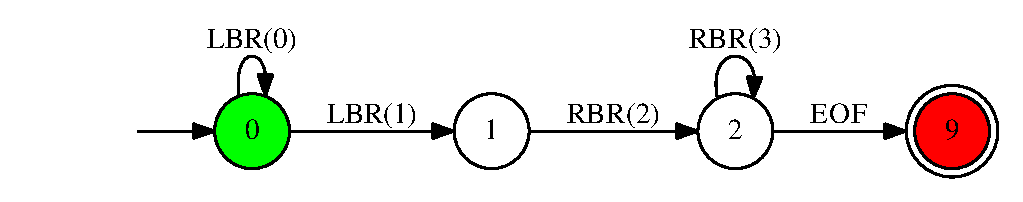
\includegraphics[scale=0.3]{dot/in3.eps}
   }  
   \hfill
    \subfloat[SPPF\label{resultSPPF}]{%
      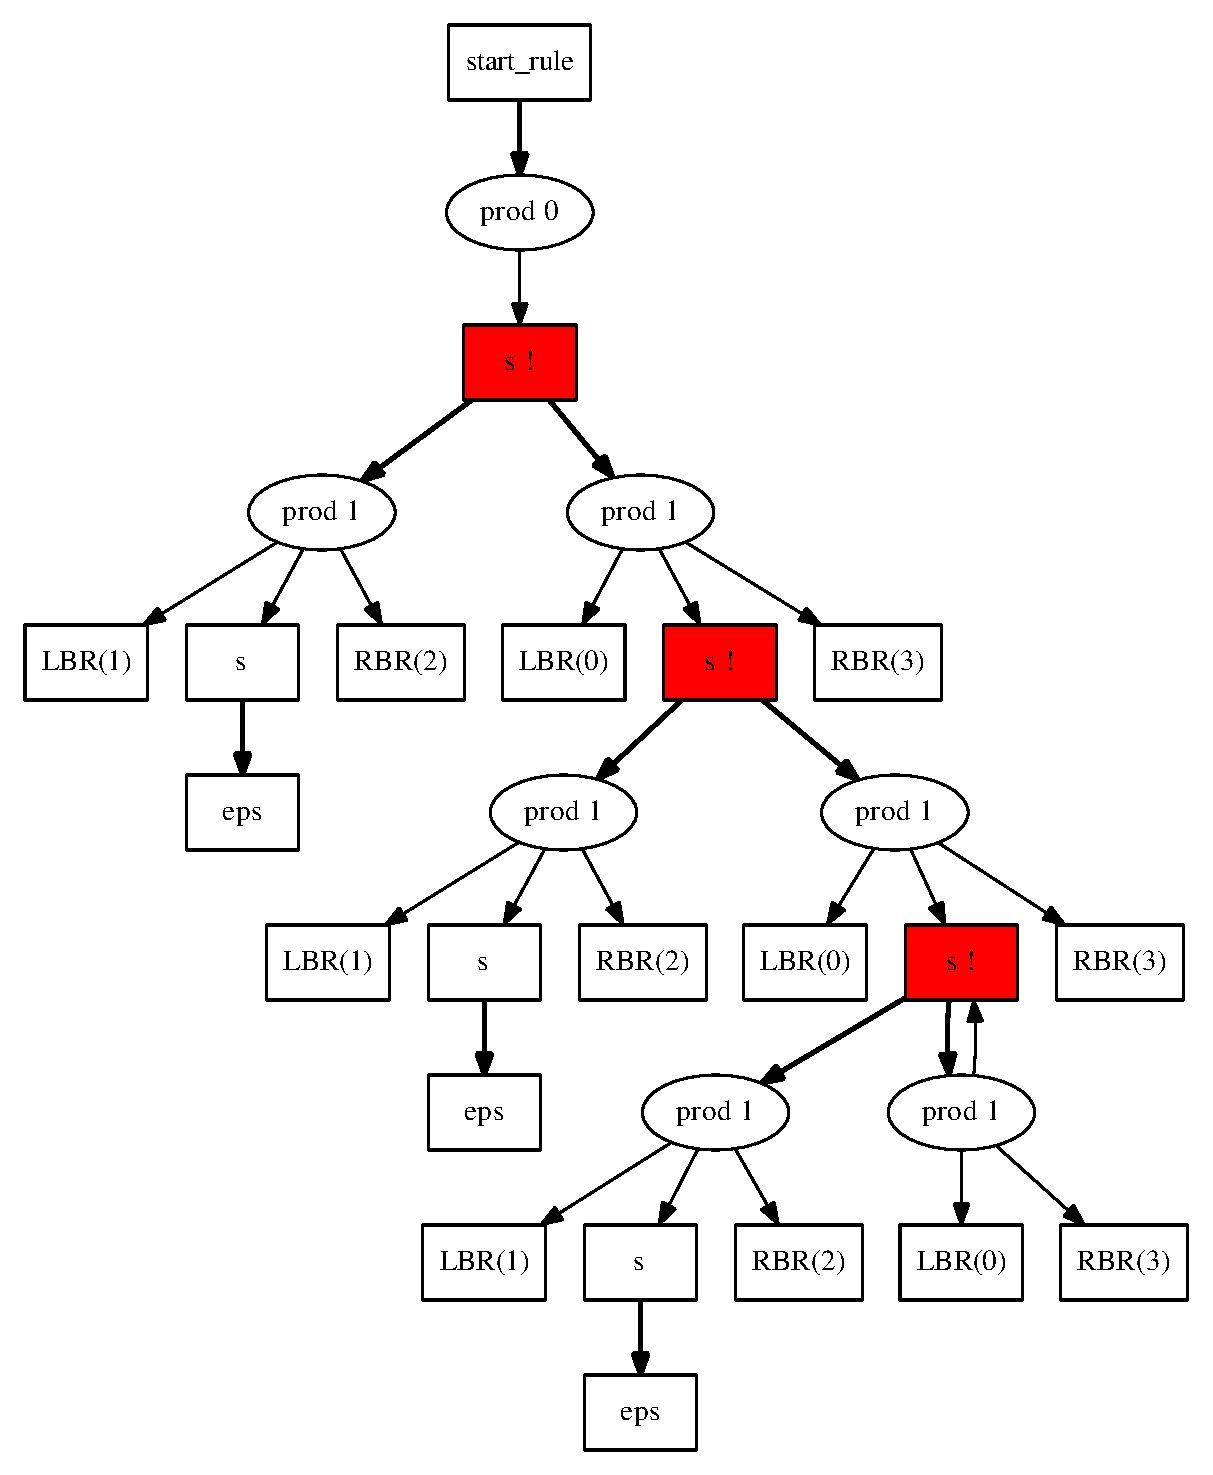
\includegraphics[scale=0.3]{dot/out3.eps}
    }
    \caption{Regular approximation and SPPF}
    \label{fig:SPPFforReg}
 \end{figure}

%\begin{figure}
%    \begin{center}
%        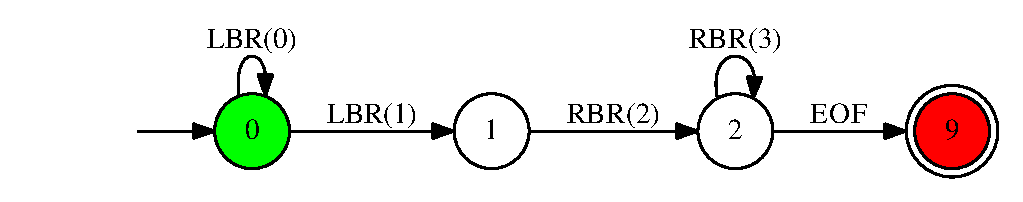
\includegraphics[scale=0.5]{dot/in3.eps}
%    \end{center}
%    \caption{$A_1$ -- input for our algorithm: regular approximation for string-embedded code after tokenization} 
%    \label{faApprox}
%\end{figure}

As it can be seen, some of the words from regular approximation do not belong to the reference language (for example, 
\verb|LBR LBR RBR|). The algorithm ignores such strings and constructs SPPF, which contains derivation trees 
for all recognized strings w.r.t. reference grammar.

%\begin{figure}
%    \begin{center}
%        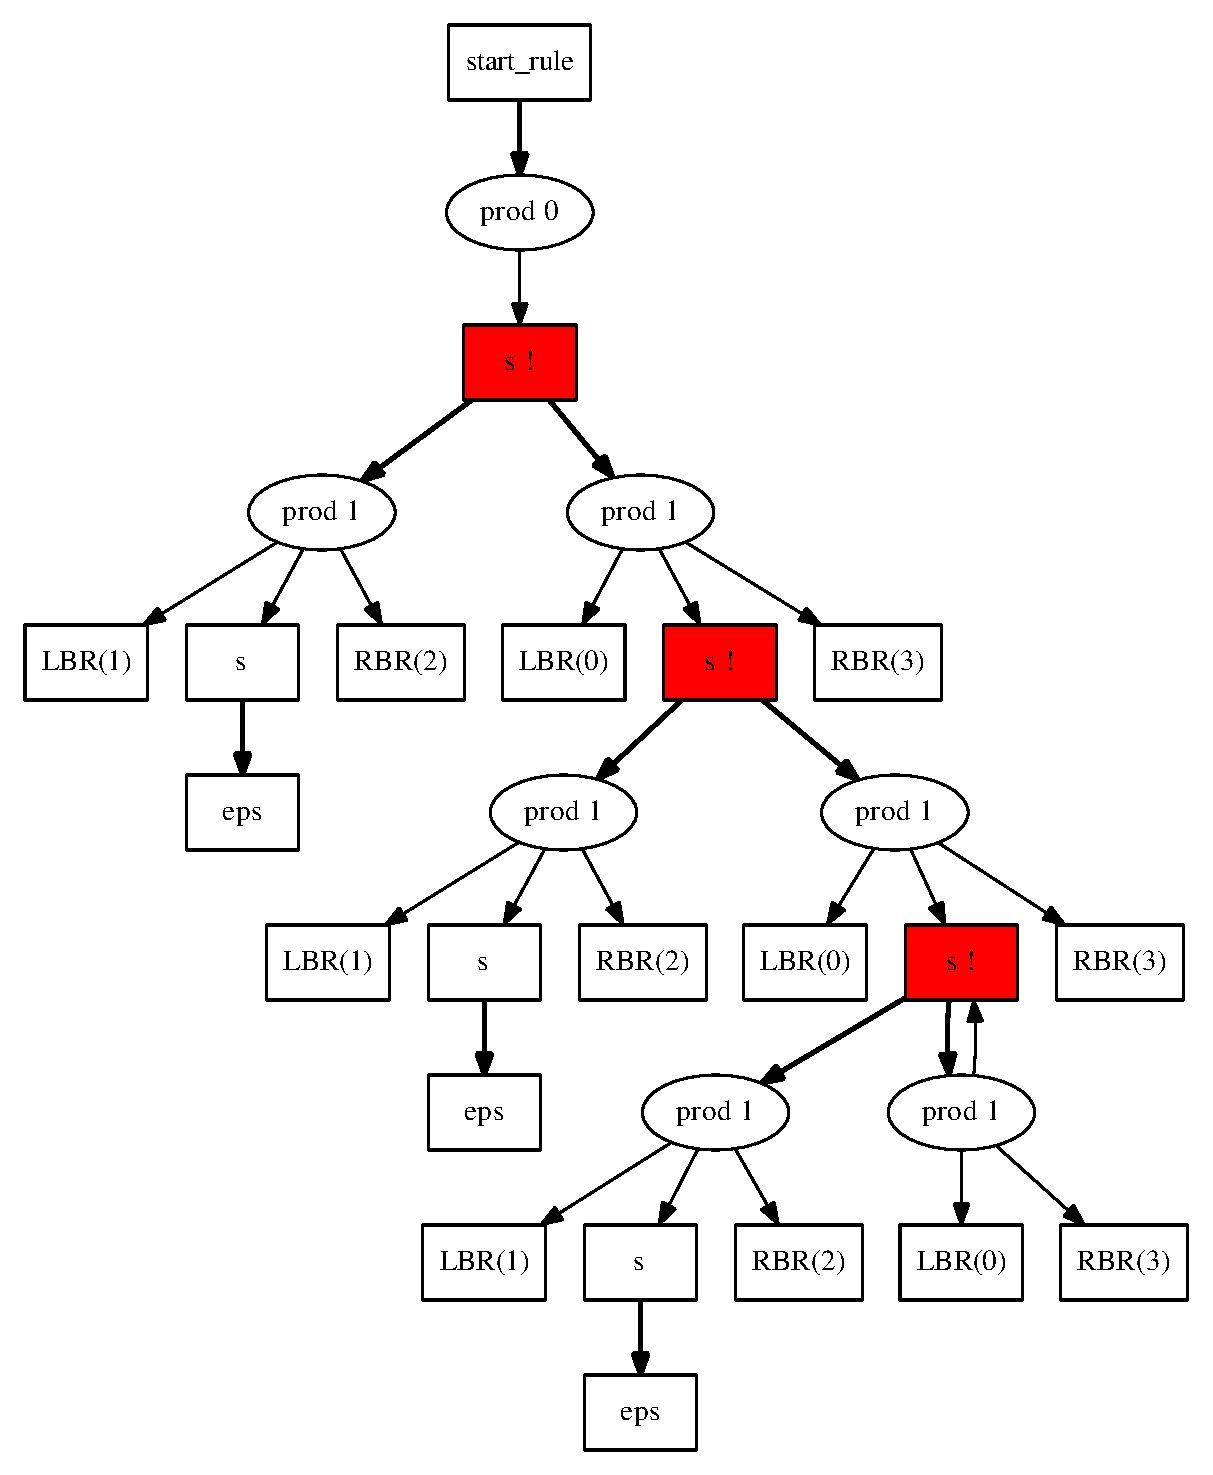
\includegraphics[scale=0.3]{dot/out3.eps}
%    \end{center}
%    \caption{SPPF for input FA presented in figure~\ref{faApprox}}
%    \label{resultSPPF}
%\end{figure}
\pagebreak
\section{\appendixname: RNGLR pseudocode}\label{RNGLRCode}

\begin{algorithm}[]
\begin{algorithmic}[1]
\caption{RNGLR algorithm}
\label{rnglr}
\Function{parse}{$grammar, input$}
  \State{$\mathcal{R} \gets \emptyset$} \Comment{Queue of tuples of GSS vertex, nonterminal, and reduction length}
  \State{$\mathcal{Q} \gets \emptyset$} \Comment{Collection of pairs of GSS vertex and parser state}
  \If{$input = \epsilon$}
    \If{$grammar$ accepts empty input} {report success}
    \Else { report failure}
    \EndIf
  \Else
    \State{\Call{addVertex}{$0, 0, startState$}}
    \ForAll{$i$ in $0..input.Length-1$}
      \State{\Call{reduce}{$i$}}
      \State{\Call{push}{$i$}}
    \EndFor
    \If{$i=input.Length-1$ and there is a vertex in the last level of GSS which state is accepting}
      \State{report success}
    \Else { report failure}
    \EndIf
  \EndIf
\EndFunction
\Function{reduce}{$i$}
  \While{$\mathcal{R}$ is not empty}
    \State{$(v, N, l) \gets \mathcal{R}.Dequeue()$}
    \State{find the set $\mathcal{X}$ of vertices reachable from $v$ along the path of length $(l-1)$}
    \State{or length $0$ if $l=0$}
    \ForAll{$v_{h} = (level_{h}, state_{h})$ in $\mathcal{X}$}
      \State{$state_{t} \gets$ calculate new state by $state_{h}$ and nonterminal $N$}
      \State{\Call{addEdge}{$i, v_{h}, v.level, state_{tail}, (l=0)$}}
    \EndFor
  \EndWhile
\EndFunction
\Function{push}{$i$}
  \State{$\mathcal{Q^{'}} \gets$ copy $\mathcal{Q}$}
  \While{$\mathcal{Q^{'}}$ is not empty}
    \State{$(v, state) \gets \mathcal{Q}.Dequeue()$}
    \State{\Call{addEdge}{$i, v, v.level + 1, state, false$}}
  \EndWhile
\EndFunction
\end{algorithmic}
\end{algorithm}

\begin{algorithm}[]
\begin{algorithmic}[1]
\caption{GSS construction}
\label{RNGLRMain}
\Function{addVertex}{$i, level, state$}
  \If{GSS does not contain vertex $v = (level, state)$}
    \State{add new vertex $v = (level, state)$ to GSS}
    \State{calculate the set of shifts by $v$ and the $input[i+1]$ and add them to $\mathcal{Q}$}
    \State{calculate the set of zero-reductions by $v$ and the $input[i+1]$ and}
    \State{add them to $\mathcal{R}$}
  \EndIf
  \State{\Return{$v$}}
\EndFunction
\Function{addEdge}{$i, v_{h}, level_{t}, state_{t}, isZeroReduction$}
  \State{$v_{t} \gets$ \Call{addVertex}{$i, level_{t}, state_{t}$}}
  \If{GSS does not contain edge from $v_{t}$ to $v_{h}$}
    \State{add new edge from $v_{t}$ to $v_{h}$ to GSS}
    \If{not $isZeroReduction$}
      \State{calculate the set of reductions by $v$ and the $input[i+1]$ and}
      \State{add them to $\mathcal{R}$}
    \EndIf
  \EndIf
\EndFunction
\end{algorithmic}
\end{algorithm}




\end{document}
